\documentclass[11pt]{article}
\usepackage{graphicx}
\usepackage{amssymb}
\usepackage{rotating}
\usepackage{authblk}
\usepackage[utf8]{inputenc}
\graphicspath{/Users/georgeadams/Dropbox/005_ITP_projects/003 TPO/GIT_repo_TPOPROJECT/}


\title{Bayesian Analysis of TPO levels in Immune Thrombocytopenia}
\author[1,2]{\small George Adams}
\author[1]{\small Adam Gosztolai}
\author[1]{\small Anwar Sayed}
\author[1]{\small Amna Malik}
\author[1]{\small Elisa Lucchini}
\author[1,2]{\small Nichola Cooper}
\affil[1]{\footnotesize Imperial College London, Kensington, London SW7 2AZ}
\affil[2]{\footnotesize Hammersmith Hospital, Imperial College NHS Trust, London W12 0HS}



\date{July 2018}

\begin{document}

\maketitle

\paragraph{Introduction:} Thrombopoietin (TPO) is a haematopoietic growth factor whose major function is in the regulation of platelet production. The exact mechanisms that regulate TPO levels are highly debated. The predominant hypothesis is that TPO is synthesised in a constitutive manner and its concentration in the blood is determined by the total volume of platelets. This is achieved by TPO binding to high-affinity receptors on the surface of platelets which then remove it from the circulation (the `sponge theory'). % As platelet counts fall, TPO levels rise, and vice-versa. %\cite{EtoLinkagemechanismsthrombocytopenia2016}. %% could try and compress this a bit  %
In patients with active ITP, TPO levels have been shown to have inappropriately low. It is believed this is because in active ITP there is a higher rate of platelet turnover which causes additional TPO to be consumed. To better understand the relationship between TPO and platelets in ITP we measured TPO levels in a 67 patients with chronic ITP and 5 patients with aplastic anaemia with a range of different platelet counts. We used aplastic anaemia as a comparator as these patients are thrombocytopenic but lack a direct immune-mediated platelet destruction. We used a bayesian regresssion model to analyse the association between TPO and platelet counts. This approach allows us to infer the probability distribution of TPO over a range of different platelet counts and has been shown to be more accurate with smaller sample sizes than classical gaussian regression models. % \cite{GoldsteinBayesiananalysisregression1976}.


\paragraph{Methods:} Blood samples were collected in duplicate in sodium citrate vacutainer tubes, double spun and stored at -80°C within four hours of collection. TPO levels were measured using quantitive sandwich enzyme immunoassay technique. We used log-normalised tpo and platelet counts in a bayesian regression model; $log(TPO) = alpha + beta*log(platelet)$. Our priors for the model where uninformative gaussian distributions (mean 0.01, standard deviation 10). We used gibbs sampling with 100,000 iterations to calculate posterior distributions from which we derived \textit{maximium a posteriori} (MAP) estimates and 90\% Bayesian Confidence intervals (BCI) for a range of platelet counts (1 to 200$x10^9/L$).


\paragraph{Results:} Of the 130 samples collected, 30 samples were excluded for failing to detect any TPO. All but 1 of these patient had a second positive sample. In the ITP group, median TPO levels was 43pg/ml (range 1.7 - 923.4pg/ml) with a median platelet count of 63$x10^9/L$ (range 3 - 328$x10^9/L$). For our Aplastic anaemia group we had 9 samples with a median TPO of 1887.6pg/ml (range 9.4-4572.5pg/ml) with a median platelet count of 20$x10^9/L$ (range 4 - 102$x10^9/L$). The higher platelet counts (\geqslant 35$x10^9/L$) in this aplastic group were from patients on tacrolimus therapy (n= 3). There was a clear non-linear relationship between platelet counts and TPO levels in both ITP and aplastic patients (FIGURE 1). At any given platelet count, MAP TPO estimates in our ITP cohort were approximately a tenth of our aplastic group. 13\% of our ITP patients were on TPOagonists, although a sensitivity analysis found this did not significantly influence model estimates. At a platelet count of 1 the MAP TPO estimate in ITP was 410pg/ml (BCI; 200-804pg/ml). This declined sharply to 100pg/ml as platelet count increased to 10$x10^9/L$. The decline in TPO became increasingly shallow as platelet counts increased, and at 100$x10^9/L$ it was 24pg/ml (BCI 18-29 pg/ml). In contrast, MAP TPO estimates in our aplastic group were \geqslant10000pg/ml at a platelet count of 1 $x10^9/L$ and 221pg/ml (BIC 112 to 828pg/ml) at 100$x10^9/L$. This is approaching the normal range for a healthy individual (mean 120pg/ml, range 80 - 230pg/ml).
% \cite{SinghCirculatingthrombopoietinlevels2015}.

%% need to put in information on treatments (22-07)


\paragraph{Conclusions:} Our study showed that in patients with ITP and aplastic anaemia there is a non-linear correlation between platelet count and TPO. The levels of TPO in our ITP patients were consistently lower than in our aplastic thrombocytopenic controls at all platelet counts. This indicates that in chronic disease, even at higher platelet counts, the immune process remains at least partially active. It also suggests that TPO, when used in this model, may be of diagnostic utility or be a potential biomarker for ITP. There is a need for such a marker in early-stage ITP to differentiate between patients who will develop chronic ITP from those who will remit, or those who have a bone marrow failure. Our group is currently undertaking a further validation study to investigate the diagnostic utility of this model.



%\begin{center}
% \begin{tabular}{||c c c c c||}
% \hline\hline
%  ITP   & platelet count & MAP & lower BCI & Upper BCI  \\
%\hline\hline
% Platelet count & 1 & 410 & 200  & 804 \\
% \hline
% Patelet count & 10 & 100 &  75 & 151 \\
% \hline
% Platelet count & 50 & 37.5 & 31 & 46 \\
% \hline
% Platelet count & 200 & 16 & 11 & 21 \\ [1ex]
% \hline
%\end{tabular}
%\end{center}

\begin{sidewaysfigure}
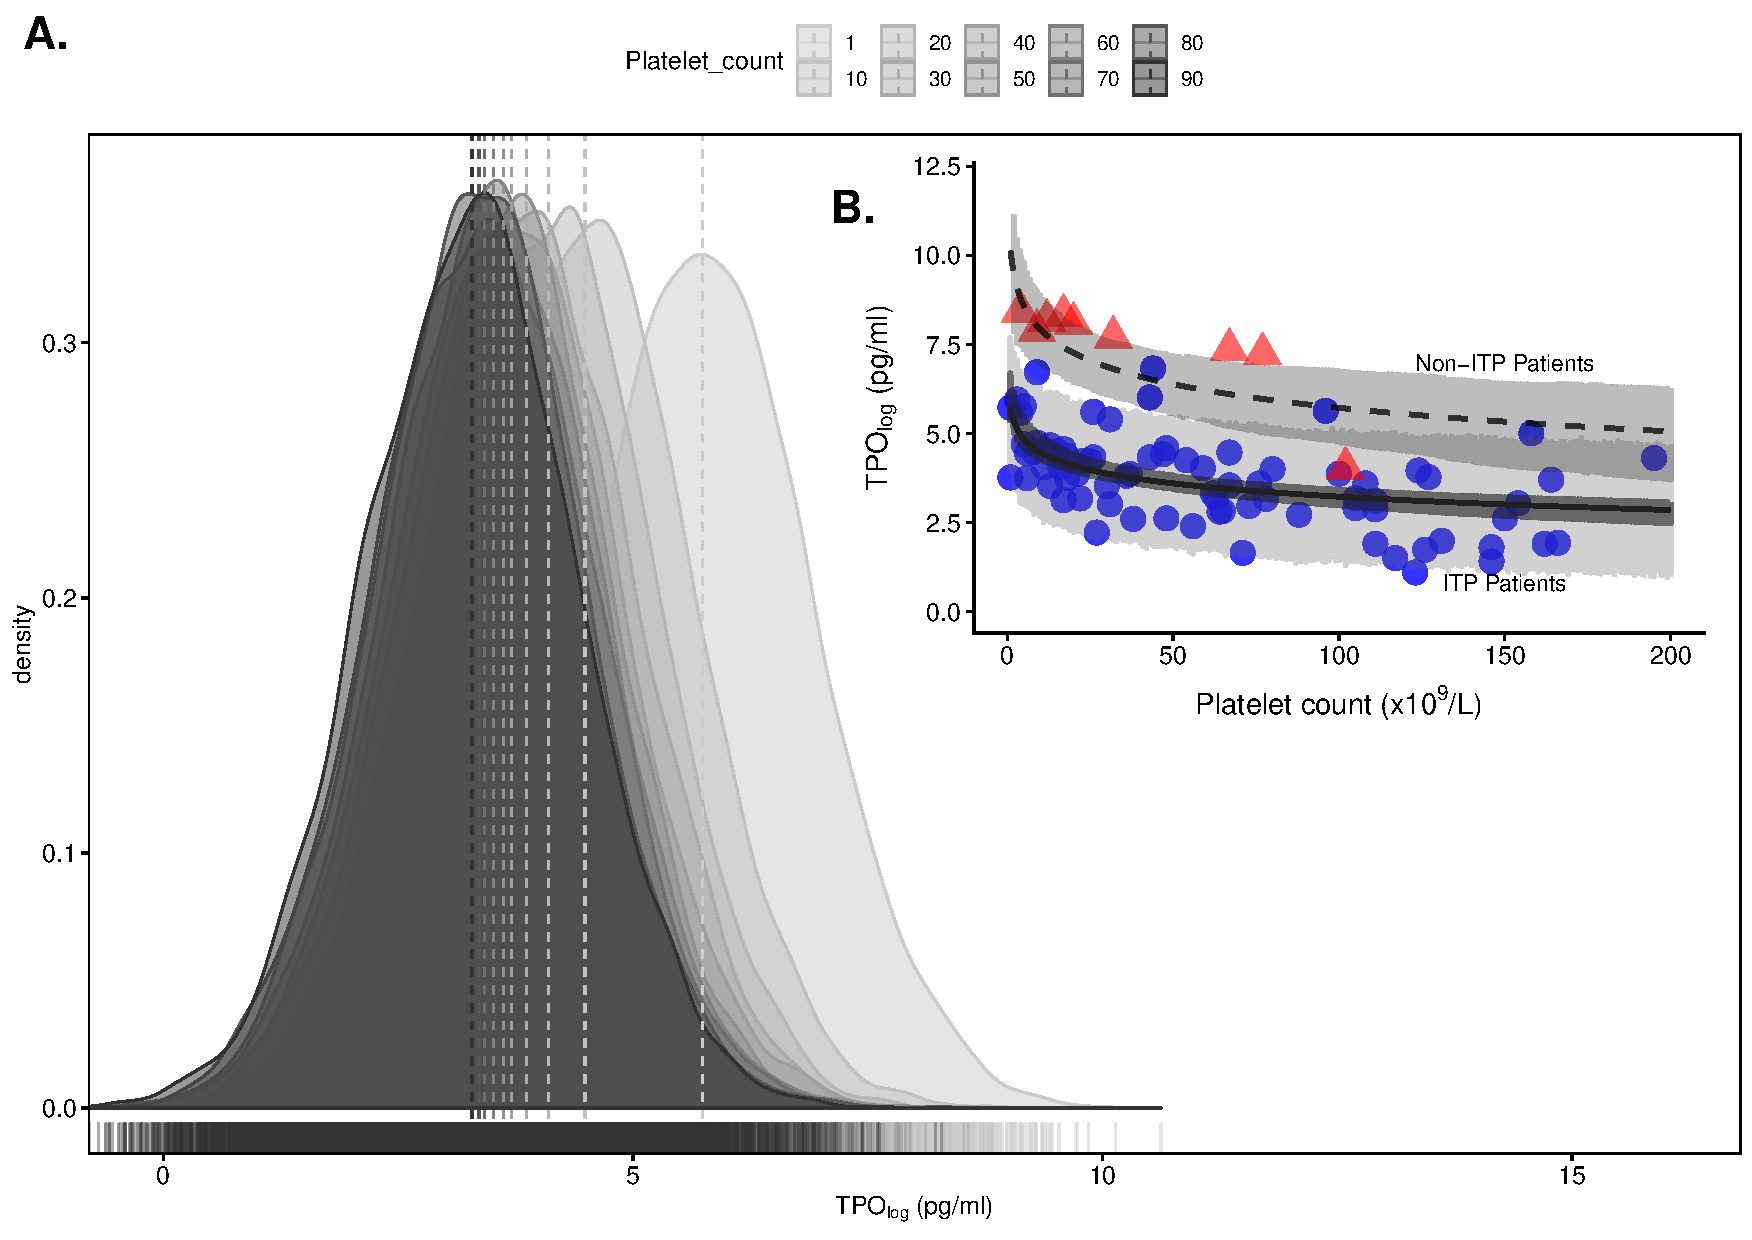
\includegraphics[width=0.8\textwidth]{ABS_v4_g1.pdf}
\caption {FIGURE 1: A.) Shows posterior probability distributions for logTPO for platelet counts ranging from 1 to 90$x10^9/L$ in our ITP patient group. Dashed vertical lines represent \textit{maximium a posteriori} (MAP) estimates for each specific platelet count, moving from right to left as platelet counts increase (and TPO levels falls). B.) Curved lines show model mean MAP estimates for logTPO levels against platelet counts in both ITP patients (lower solid line) and aplastic controls (upper dashed line). Points represent the individual results for the ITP patients, and Triangles represent Aplastic patients. Darker shaded area represent the 90\% bayesian credible interval (BCI) and the lighter shading represents the simulated observational interval}
\end{sidewaysfigure}

\bibliographystyle{plain}
\bibliography{tpobib.bib}


\paragraph{}
\textbf{Currently 3804 characters - needs to be characters: 3800}


\end{document}
